\documentclass[11pt,letterpaper]{article}
\usepackage[utf8]{inputenc}
\usepackage[T1]{fontenc}
\usepackage{lmodern}
\usepackage[margin=1in]{geometry}
\usepackage{amsmath,amssymb,amsfonts,amsthm}
\usepackage{booktabs}
\usepackage{microtype}
\usepackage{enumitem}
\usepackage{fancyhdr}
\usepackage{titlesec}
\usepackage{xcolor}
\usepackage{tikz}
\usepackage{pgfplots}
\usepackage{mdframed}
\usepackage[hidelinks,colorlinks=true,linkcolor=SlateBlue,citecolor=SlateBlue,urlcolor=Terracotta]{hyperref}

\pgfplotsset{compat=1.18}
\usetikzlibrary{arrows.meta,positioning,calc,patterns,decorations.pathreplacing}

\definecolor{SlateBlue}{HTML}{1E293B}
\definecolor{Terracotta}{HTML}{C2410C}
\definecolor{ForestGreen}{HTML}{15803D}
\definecolor{LightSlate}{HTML}{F8FAFC}
\definecolor{BorderGray}{HTML}{CBD5E1}
\definecolor{LightTerracotta}{HTML}{FFF7ED}
\definecolor{CourseBlue}{HTML}{0072B2}
\definecolor{CourseOrange}{HTML}{D55E00}
\definecolor{CourseTeal}{HTML}{009E73}
\definecolor{CoursePurple}{HTML}{CC79A7}
\definecolor{CourseAmber}{HTML}{E69F00}

\titleformat{\section}{\normalfont\Large\bfseries\color{SlateBlue}}{\thesection}{1em}{}[\titlerule]
\titleformat{\subsection}{\normalfont\large\bfseries\color{SlateBlue}}{\thesubsection}{1em}{}
\titleformat{\subsubsection}{\normalfont\normalsize\bfseries\color{Terracotta}}{\thesubsubsection}{1em}{}

\pagestyle{fancy}
\fancyhf{}
\renewcommand{\headrulewidth}{0.4pt}
\renewcommand{\footrulewidth}{0.4pt}
\fancyhead[L]{\small\scshape\color{SlateBlue}\leftmark}
\fancyhead[R]{\small\color{SlateBlue}Principles of Economics}
\fancyfoot[C]{\thepage}

\newmdenv[
  linecolor=Terracotta,
  linewidth=1.5pt,
  backgroundcolor=LightTerracotta,
  innertopmargin=10pt,
  innerbottommargin=10pt,
  innerrightmargin=12pt,
  innerleftmargin=12pt,
  roundcorner=4pt,
  skipabove=12pt,
  skipbelow=12pt
]{coreprinciple}

\newmdenv[
  linecolor=SlateBlue,
  linewidth=1.5pt,
  backgroundcolor=LightSlate,
  innertopmargin=10pt,
  innerbottommargin=10pt,
  innerrightmargin=12pt,
  innerleftmargin=12pt,
  roundcorner=4pt,
  skipabove=12pt,
  skipbelow=12pt
]{casestudy}

\newenvironment{examplecase}[1]{%
  \begin{casestudy}
  \boxheader{SlateBlue}{#1}
  \vspace{0.4em}
}{%
  \end{casestudy}
}

\newmdenv[
  linecolor=BorderGray,
  linewidth=1pt,
  backgroundcolor=white,
  innertopmargin=10pt,
  innerbottommargin=10pt,
  innerrightmargin=12pt,
  innerleftmargin=12pt,
  roundcorner=4pt,
  skipabove=12pt,
  skipbelow=12pt
]{takeaways}

\newcommand{\boxheader}[2]{{\noindent\bfseries\color{#1}\Large #2}\vspace{0.4em}\par}

% ==============================================================================
% TikZ & PGFPlots Global Configuration and Economics Styling
% ==============================================================================

\usepackage{tikz}
\usepackage{pgfplots}
\pgfplotsset{compat=1.18}

% TikZ Libraries
\usetikzlibrary{
    arrows.meta,
    positioning,
    calc,
    shapes.geometric,
    patterns,
    decorations.pathreplacing,
    intersections
}

% Common Economics TikZ Styles
\tikzset{
    % Axes and Structural Lines
    econ axis/.style={->, >=Stealth, thick, color=SlateBlue!90!black},
    econ grid/.style={thin, dashed, color=gray!30},
    econ guide/.style={dashed, color=gray!60, thin},
    % Curves and Functions
    demand curve/.style={very thick, color=SlateBlue},
    supply curve/.style={very thick, color=Terracotta},
    mb curve/.style={very thick, color=SlateBlue},
    mc curve/.style={very thick, color=Terracotta},
    % Points and Highlights
    econ point/.style={circle, fill=SlateBlue!90!black, inner sep=1.8pt},
    econ highlight/.style={fill=Terracotta!20, opacity=0.5},
    % Annotations
    econ label/.style={font=\small\sffamily, align=center},
    econ annotation/.style={font=\footnotesize\itshape, color=SlateBlue!80!black}
}

% PGFPlots Standard Economics Style
\pgfplotsset{
    econ diagram/.style={
        axis lines=left,
        xlabel style={at={(ticklabel* cs:1)}, anchor=north west, font=\small\bfseries},
        ylabel style={at={(ticklabel* cs:1)}, anchor=south east, font=\small\bfseries},
        label style={font=\small},
        tick label style={font=\small},
        grid=none,
        enlargelimits=false,
        axis line style={->, >=Stealth, thick, color=SlateBlue!90!black}
    }
}

\usepackage{tcolorbox}

\begin{document}

\title{\Huge\bfseries\color{SlateBlue} Chapter 14: International Trade, Comparative Advantage, and Protectionism}
\author{\large Principles of Microeconomics Curriculum}
\date{Spring 2027}
\maketitle

\thispagestyle{plain}

\begin{abstract}
This chapter applies supply, demand, and welfare economics to international trade. Using the small open economy model, we trace how opening to trade creates net social surplus gains alongside sharp distributional splits between domestic consumers and producers, analyze the welfare transfers and deadweight losses of tariffs and import quotas, and evaluate classic arguments for trade protection.
\end{abstract}

\tableofcontents
\vspace{1.5em}
\hrule
\vspace{1.5em}

\begin{examplecase}{Bring It Home: Why Do Steel Tariffs Spark Fierce Debate Between Steelworkers and Automakers?}
Whenever a government proposes a tariff on imported steel, two groups immediately take opposite sides. Domestic steel mills and factory workers argue that tariffs protect domestic manufacturing jobs and sustain vital industrial capacity. Meanwhile, downstream manufacturers---automakers, appliance makers, and construction firms---along with everyday households warn that tariffs act as a hidden tax that raises the cost of cars, buildings, and consumer goods. How can a single border tax feel like an economic lifeline to one group and a costly burden to millions of others? Throughout this chapter, we use consumer surplus, producer surplus, and deadweight loss to account for every dollar of gains, transfers, and permanent economic waste under free trade and protectionism.
\end{examplecase}

% -----------------------------------------------------------------------------
% Section 14.1: Comparative Advantage and Free Trade Welfare Mechanics
% -----------------------------------------------------------------------------
\section{Comparative Advantage and Free Trade Welfare Mechanics}

\subsection*{Conceptual Introduction}
In Chapter 2, we used the production possibilities frontier (PPF) to show that when countries specialize according to \textbf{comparative advantage}---producing goods at a lower domestic opportunity cost---and trade, total consumption can expand beyond domestic production limits. Now we bring comparative advantage into a single-market supply-and-demand framework to pinpoint \emph{who wins and who loses} inside a country when it opens its borders to international trade. Throughout our core graphical and algebraic analysis, we assume a \textbf{small open economy} (the country is a price-taker in the world market and cannot alter the global price), linear domestic supply and demand curves, competitive markets, and zero transportation costs (\emph{ceteris paribus}).

To determine whether a small open economy becomes an importer or an exporter of a specific good, compare its \textbf{autarky (no-trade) domestic equilibrium price ($P_A$)} against the prevailing \textbf{world price ($P_w$)}:
\begin{itemize}
    \item \textbf{Importing Country ($P_w < P_A$):} Foreign producers have a comparative advantage and can supply the good at a lower opportunity cost than domestic firms. Under free trade, the domestic price drops from $P_A$ to $P_w$. Domestic consumers benefit---buying more at a lower price and capturing a large expansion in \textbf{Consumer Surplus ($CS$)}. Domestic producers are harmed---cutting production and losing \textbf{Producer Surplus ($PS$)}. Crucially, the gain to consumers strictly exceeds the loss to domestic producers, creating a net gain in \textbf{Total Social Surplus ($TS = CS + PS$)}.
    \item \textbf{Exporting Country ($P_w > P_A$):} Domestic producers have a comparative advantage and can sell abroad at a higher world price. Under free trade, the domestic price rises from $P_A$ to $P_w$. Domestic producers expand output and capture a gain in Producer Surplus that strictly exceeds the loss in Consumer Surplus suffered by domestic buyers---once again generating a positive net gain in Total Social Surplus.
\end{itemize}

This sharp distributional split explains why trade policy is perpetually contentious in real-world markets such as global apparel, consumer electronics, and agricultural exports. When households buy smartphones, laptops, and clothing sourced from specialized global supply chains at lower world prices, the gains from free trade are spread thinly across millions of consumers (for example, saving $\$30$ on a pair of shoes). By contrast, the losses from import competition are concentrated among specific domestic factories and workers, giving import-competing industries a strong incentive to lobby for trade barriers even when free trade expands total national surplus.

\begin{tcolorbox}[colback=CourseAmber!10!white,colframe=CourseOrange,title=\textbf{Clear It Up: Do Imports Subtract from National Welfare Because Domestic Producers Lose?}]
A common misconception is that exports are always ``good'' for an economy while imports are ``bad'' because imports reduce domestic producer surplus in the competing industry. In welfare economics, \emph{both} exporting and importing raise Total Social Surplus. When a country imports at $P_w < P_A$, domestic consumers gain more surplus than domestic producers lose ($\Delta CS + \Delta PS = \Delta TS > 0$), and domestic labor and capital are freed to move toward sectors where the country holds a comparative advantage.
\end{tcolorbox}

\subsection*{Visual Representation}
Figure~\ref{fig:free_trade_imports} illustrates an importing market where the world price $P_w = \$40$ lies below the autarky price $P_A = \$60$, expanding Total Social Surplus by the shaded teal triangle. Table~\ref{tab:free_trade_summary} summarizes how both importing and exporting reshape domestic prices and surplus.

\begin{figure}[htbp]
\centering
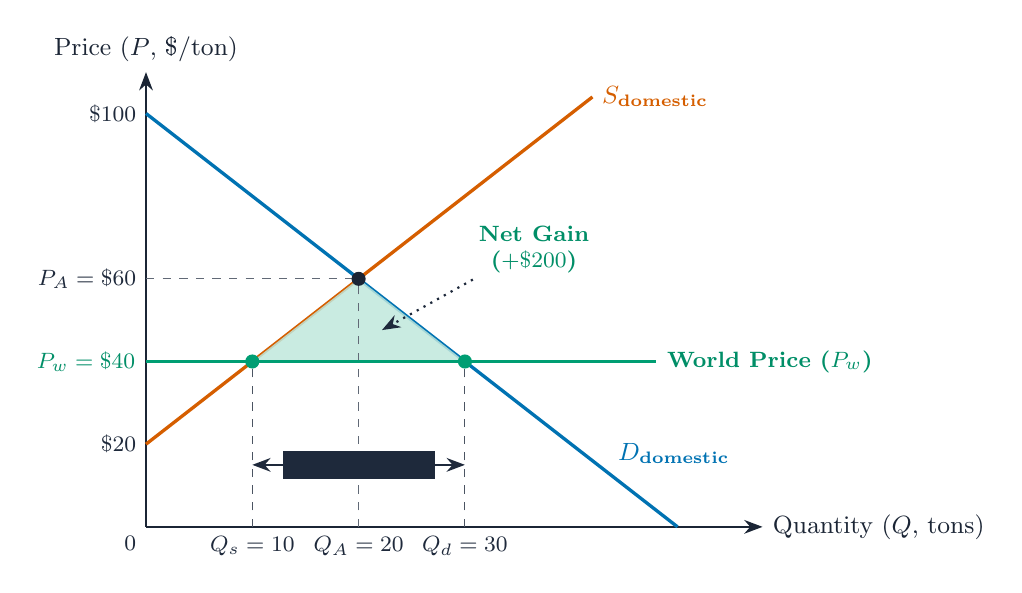
\begin{tikzpicture}[xscale=1.35, yscale=1.05]
    % Axes
    \draw[econ axis] (0,0) -- (5.8,0) node[right, font=\small] {Quantity ($Q$, tons)};
    \draw[econ axis] (0,0) -- (0,5.5) node[above, font=\small] {Price ($P$, \$/ton)};
    \node[below left, font=\footnotesize, color=SlateBlue] at (0,0) {$0$};

    % Demand: P = 100 - 2Q -> (0,5) to (5,0); Supply: P = 20 + 2Q -> (0,1) to (4.25,5.25)
    % Autarky E_A(20, $60) -> (2.0, 3.0)
    \draw[very thick, color=CourseBlue] (0,5.0) -- (5.0,0);
    \node[above right, font=\small\bfseries, color=CourseBlue] at (4.35,0.65) {$D_{\text{domestic}}$};
    \draw[very thick, color=CourseOrange] (0,1.0) -- (4.2,5.2);
    \node[right, font=\small\bfseries, color=CourseOrange] at (4.2,5.2) {$S_{\text{domestic}}$};

    % Vertical axis intercepts
    \node[left, font=\footnotesize, color=SlateBlue] at (0,5.0) {$\$100$};
    \node[left, font=\footnotesize, color=SlateBlue] at (0,1.0) {$\$20$};

    % Net Gains from Trade Triangle: (1,2) to (3,2) to (2,3)
    \fill[CourseTeal!25, opacity=0.85] (1.0,2.0) -- (3.0,2.0) -- (2.0,3.0) -- cycle;

    % Autarky reference drop-lines
    \draw[dashed, color=SlateBlue!70] (0,3.0) node[left, font=\footnotesize, color=SlateBlue] {$P_A = \$60$} -- (2.0,3.0);
    \draw[dashed, color=SlateBlue!70] (2.0,0) node[below, font=\footnotesize, color=SlateBlue] {$Q_A = 20$} -- (2.0,3.0);

    % World Price Pw = $40 (y = 2.0): Qs = 10 (x=1.0), Qd = 30 (x=3.0), Imports = 20
    \draw[very thick, color=CourseTeal] (0,2.0) node[left, font=\footnotesize\bfseries, color=CourseTeal!90!black] {$P_w = \$40$} -- (4.8,2.0) node[right, font=\footnotesize\bfseries, color=CourseTeal!90!black] {World Price ($P_w$)};
    \draw[dashed, color=SlateBlue!80] (1.0,0) node[below, font=\footnotesize, color=SlateBlue] {$Q_s = 10$} -- (1.0,2.0);
    \draw[dashed, color=SlateBlue!80] (3.0,0) node[below, font=\footnotesize, color=SlateBlue] {$Q_d = 30$} -- (3.0,2.0);

    % Equilibrium and trade points
    \node[econ point] at (2.0,3.0) {};
    \node[econ point, fill=CourseTeal] at (1.0,2.0) {};
    \node[econ point, fill=CourseTeal] at (3.0,2.0) {};

    % Clean leader callout for Net Gain (zero text-on-line)
    \node[font=\footnotesize\bfseries, color=CourseTeal!90!black, fill=white, inner sep=2pt, align=center] (netgain) at (3.65,3.35) {Net Gain\\($+\$200$)};
    \draw[dotted, thick, color=SlateBlue, ->, >=Stealth] (netgain.south west) -- (2.22,2.38);

    % Imports bracket with opaque white background over the Q_A drop-line
    \draw[<->, >=Stealth, thick, color=SlateBlue] (1.0,0.75) -- node[fill=white, inner sep=2pt, font=\scriptsize\bfseries, color=SlateBlue] {Imports $= 20$} (3.0,0.75);
\end{tikzpicture}
\caption{Welfare Gains from Free Trade (Importing Case). When $P_w = \$40 < P_A = \$60$, domestic production falls from $20$ to $10$ tons and domestic consumption rises from $20$ to $30$ tons, generating $20$ tons of imports and a net gain in Total Social Surplus (shaded teal triangle).}
\label{fig:free_trade_imports}
\end{figure}

\begin{table}[htbp]
\centering
\caption{Free Trade Welfare Direction in a Small Open Economy}
\label{tab:free_trade_summary}
\begin{tabular}{lcccc}
\toprule
\textbf{Trade Regime} & \textbf{Domestic Price} & \textbf{$\Delta CS$} & \textbf{$\Delta PS$} & \textbf{$\Delta TS = \Delta CS + \Delta PS$} \\
\midrule
Importing Country ($P_w < P_A$) & Falls ($P_A \to P_w$) & Increases ($+$) & Decreases ($-$) & Increases ($+$) \\
Exporting Country ($P_w > P_A$) & Rises ($P_A \to P_w$) & Decreases ($-$) & Increases ($+$) & Increases ($+$) \\
\bottomrule
\end{tabular}
\end{table}

\subsection*{Mathematical Foundation (Algebra-First)}
Assuming linear domestic demand and supply in a small open economy, trade volumes and net social surplus gains are computed directly using triangle areas:
\begin{equation}
\text{Importing } (P_w < P_A): \quad \text{Imports} = Q_d(P_w) - Q_s(P_w), \qquad \Delta TS_{\text{import}} = \frac{1}{2} \times \text{Imports} \times (P_A - P_w)
\end{equation}
\begin{equation}
\text{Exporting } (P_w > P_A): \quad \text{Exports} = Q_s(P_w) - Q_d(P_w), \qquad \Delta TS_{\text{export}} = \frac{1}{2} \times \text{Exports} \times (P_w - P_A)
\end{equation}

\begin{tcolorbox}[colback=LightSlate,colframe=CourseBlue,title=\textbf{Work It Out 14.1: Free Trade Surplus in a Small Steel Market}]
In a small open economy's market for steel, domestic inverse demand is $P = 100 - 2Q_d$ and domestic inverse supply is $P = 20 + 2Q_s$, where $P$ is measured in dollars per ton and $Q$ in tons.
\begin{enumerate}
    \item Find the autarky equilibrium price $P_A$, quantity $Q_A$, and autarky surplus ($CS_A$, $PS_A$, $TS_A$).
    \item Suppose the country opens to free trade at a world price of $P_w = \$40$ per ton. Calculate domestic quantity supplied, domestic quantity demanded, import volume, $\Delta CS$, $\Delta PS$, and the net gain in Total Social Surplus ($\Delta TS$).
    \item \emph{Exporting Check:} What would happen to trade volume and $\Delta TS$ if the world price were instead $P_w = \$80$ per ton?
\end{enumerate}

\medskip
\noindent\textbf{Step-by-Step Solution:}
\begin{enumerate}
    \item \textbf{Autarky Equilibrium ($P_A, Q_A$) and Autarky Surplus:}
    Set inverse demand equal to inverse supply ($Q_d = Q_s = Q_A$):
    \[
    100 - 2Q_A = 20 + 2Q_A \implies 80 = 4Q_A \implies Q_A = \mathbf{20\text{ tons}}, \qquad P_A = 100 - 2(20) = \mathbf{\$60}
    \]
    Using the vertical intercepts ($\$100$ for demand and $\$20$ for supply):
    \[
    CS_A = \frac{1}{2}(20)(\$100 - \$60) = \$400, \qquad PS_A = \frac{1}{2}(20)(\$60 - \$20) = \$400, \qquad TS_A = \mathbf{\$800}
    \]

    \item \textbf{Importing Equilibrium at $P_w = \$40$:}
    \[
    40 = 20 + 2Q_s \implies 2Q_s = 20 \implies Q_s = \mathbf{10\text{ tons produced domestically}}
    \]
    \[
    40 = 100 - 2Q_d \implies 2Q_d = 60 \implies Q_d = \mathbf{30\text{ tons consumed domestically}}
    \]
    \[
    \text{Imports} = Q_d - Q_s = 30 - 10 = \mathbf{20\text{ tons}}
    \]
    Compute free-trade Consumer and Producer Surplus:
    \[
    CS_{\text{trade}} = \frac{1}{2}(30)(\$100 - \$40) = \$900 \implies \Delta CS = \$900 - \$400 = \mathbf{+\$500}
    \]
    \[
    PS_{\text{trade}} = \frac{1}{2}(10)(\$40 - \$20) = \$100 \implies \Delta PS = \$100 - \$400 = \mathbf{-\$300}
    \]
    Verify Net Social Surplus Gain two ways:
    \[
    \Delta TS = \Delta CS + \Delta PS = +\$500 - \$300 = \mathbf{+\$200}
    \]
    \[
    \Delta TS = \frac{1}{2} \times \text{Imports} \times (P_A - P_w) = \frac{1}{2} \times 20 \times (\$60 - \$40) = 10 \times \$20 = \mathbf{+\$200}
    \]

    \item \textbf{Exporting Check at $P_w = \$80$:}
    Since $P_w = \$80 > P_A = \$60$, the country becomes an exporter:
    \[
    80 = 20 + 2Q_s \implies Q_s = 30\text{ tons}, \qquad 80 = 100 - 2Q_d \implies Q_d = 10\text{ tons}
    \]
    \[
    \text{Exports} = Q_s - Q_d = 30 - 10 = \mathbf{20\text{ tons}}
    \]
    Here $CS_{\text{exp}} = \frac{1}{2}(10)(100 - 80) = \$100$ ($\Delta CS = -\$300$) and $PS_{\text{exp}} = \frac{1}{2}(30)(80 - 20) = \$900$ ($\Delta PS = +\$500$), yielding the exact same net gain $\Delta TS = \frac{1}{2}(20)(\$80 - \$60) = \mathbf{+\$200}$.
\end{enumerate}
\textbf{Conclusion:} Opening to free trade raises national social welfare by $+\$200$ whether the country imports at $\$40$ or exports at $\$80$, though the domestic winners and losers flip between the two cases.
\end{tcolorbox}

\begin{tcolorbox}[colback=SlateBlue!5!white,colframe=SlateBlue,title=\textbf{Optional Advanced Calculus Extension: Integral Form of Gains from Trade}]
\small
\emph{Note for Economics Majors and Quantitative Students:}
For general (possibly nonlinear) domestic demand $Q_d(P)$ and supply $Q_s(P)$, welfare changes under importing ($P_w < P_A$) are exact definite integrals with respect to price:
\[
\Delta CS = \int_{P_w}^{P_A} Q_d(P)\,dP, \qquad \Delta PS = -\int_{P_w}^{P_A} Q_s(P)\,dP, \qquad \Delta TS = \int_{P_w}^{P_A} \bigl[Q_d(P) - Q_s(P)\bigr]\,dP.
\]
In our steel market, inverting the linear curves gives $Q_d(P) = 50 - 0.5P$ and $Q_s(P) = 0.5P - 10$, so import demand is $M(P) = Q_d(P) - Q_s(P) = 60 - P$. Integrating from $P_w = 40$ to $P_A = 60$ confirms our geometric triangle:
\[
\Delta TS = \int_{40}^{60} (60 - P)\,dP = \left[60P - \frac{1}{2}P^2\right]_{40}^{60} = (3{,}600 - 1{,}800) - (2{,}400 - 800) = 1{,}800 - 1{,}600 = +\$200.
\]
\end{tcolorbox}

% -----------------------------------------------------------------------------
% Section 14.2: Tariffs, Import Quotas, and Deadweight Loss
% -----------------------------------------------------------------------------
\section{Tariffs, Import Quotas, and Deadweight Loss}

\subsection*{Conceptual Introduction}
To shield domestic industries from foreign competition, governments frequently impose trade barriers---most commonly a \textbf{tariff} (a per-unit or percentage tax levied on imported goods) or an \textbf{import quota} (a legal cap on the physical quantity of a good allowed to enter the country). In our small open economy benchmark, foreign supply at the world price $P_w$ is perfectly elastic, so imposing a per-unit tariff $t$ raises the domestic market price by the full amount of the tariff, from $P_w$ to $P_t = P_w + t$.

This price increase triggers four distinct welfare effects relative to free trade, traditionally labeled Areas $A, B, C,$ and $D$:
\begin{itemize}
    \item \textbf{Consumer Surplus Shrinks by $-(A + B + C + D)$:} Domestic buyers pay a higher price ($P_w + t$) and cut consumption from $Q_{d1}$ to $Q_{d2}$.
    \item \textbf{Producer Surplus Expands by $+A$:} Protected by the higher domestic price, domestic producers expand output from $Q_{s1}$ to $Q_{s2}$. Area $A$ is a direct transfer from domestic consumers to domestic firms.
    \item \textbf{Government Tariff Revenue Equals $+C = t \times (Q_{d2} - Q_{s2})$:} The domestic treasury collects $t$ dollars on every imported unit that still crosses the border.
    \item \textbf{Deadweight Loss Equals $-(B + D)$:} Area $B$ represents \textbf{production inefficiency} (using higher-cost domestic resources to produce units that could have been imported cheaply at $P_w$), while Area $D$ represents \textbf{consumption inefficiency} (mutually beneficial trades lost when buyers whose willingness to pay exceeds $P_w$ are priced out at $P_w + t$).
\end{itemize}

An \textbf{import quota} restricting imports to the exact same volume ($Q_{d2} - Q_{s2}$) pushes the domestic price to the same level $P_w + t$ and causes the exact same deadweight loss $(B + D)$---with one critical difference. Instead of generating domestic tax revenue, Area $C$ becomes \textbf{quota rents} captured by whoever holds the valuable \textbf{import licenses}. If licenses are given away to foreign exporters (as under a voluntary export restraint), Area $C$ flows abroad, increasing the importing country's net welfare loss from $B + D$ to $B + C + D$. In practice, when tariffs or quotas raise the domestic price of intermediate inputs such as steel or solar panels, domestic producers capture Area $A$, while downstream manufacturers---such as automakers, construction firms, and rooftop solar installers---face higher input costs that squeeze margins and raise retail prices.

\begin{tcolorbox}[colback=CourseAmber!10!white,colframe=CourseOrange,title=\textbf{Clear It Up: Why Tariffs Create Two Deadweight Loss Triangles ($B + D$)}]
Unlike a domestic excise tax (which creates a single Harberger deadweight loss triangle), an import tariff creates \emph{two} separate deadweight loss triangles. \textbf{Triangle $B$} wastes productive resources by pulling higher-cost domestic suppliers into production above $P_w$, while \textbf{Triangle $D$} destroys consumer surplus by pricing out domestic buyers who value the good above $P_w$ but below $P_w + t$.
\end{tcolorbox}

\subsection*{Visual Representation}
Figure~\ref{fig:tariff_welfare} illustrates the four welfare regions ($A, B, C, D$) created when a per-unit tariff of $t = \$10$ raises the domestic steel price from $P_w = \$40$ to $P_w + t = \$50$. Table~\ref{tab:tariff_vs_quota} compares the welfare incidence of a tariff against an equivalent import quota.

\begin{figure}[htbp]
\centering
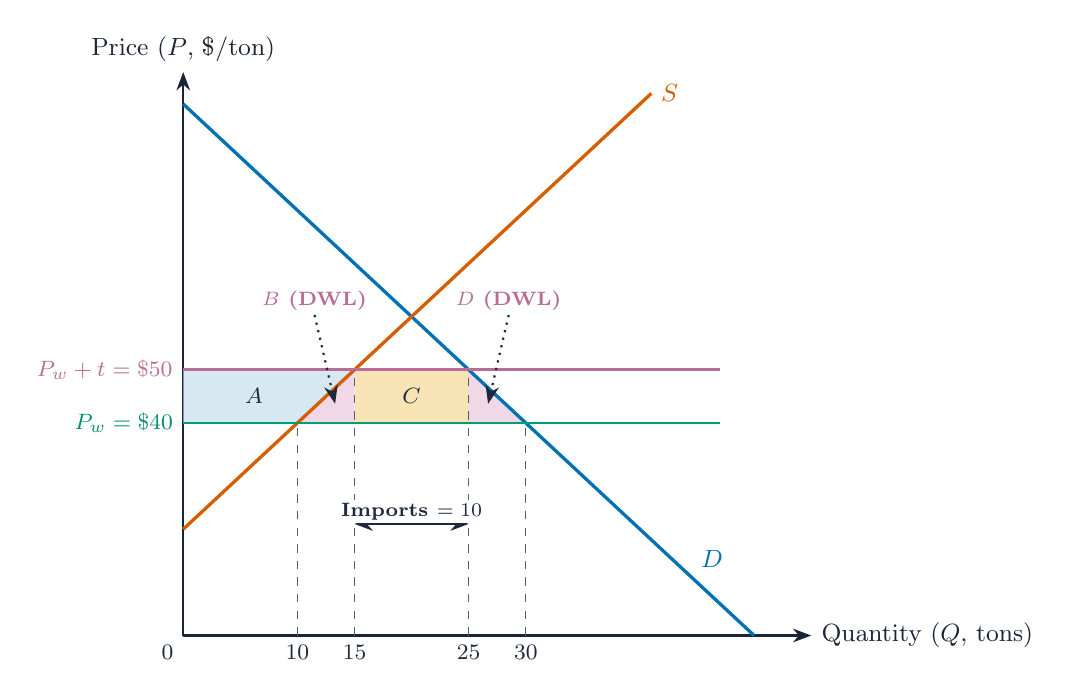
\begin{tikzpicture}[xscale=1.45, yscale=1.35]
    % Axes
    \draw[econ axis] (0,0) -- (5.5,0) node[right, font=\small] {Quantity ($Q$, tons)};
    \draw[econ axis] (0,0) -- (0,5.3) node[above, font=\small] {Price ($P$, \$/ton)};
    \node[below left, font=\footnotesize, color=SlateBlue] at (0,0) {$0$};

    % Shaded Welfare Regions
    % Area A: Producer Surplus gain trapezoid (0,2) -> (1,2) -> (1.5,2.5) -> (0,2.5)
    \fill[CourseBlue!18, opacity=0.9] (0,2.0) -- (1.0,2.0) -- (1.5,2.5) -- (0,2.5) -- cycle;
    % Area B: DWL left triangle (1,2) -> (1.5,2) -> (1.5,2.5)
    \fill[CoursePurple!32, opacity=0.9] (1.0,2.0) -- (1.5,2.0) -- (1.5,2.5) -- cycle;
    % Area C: Tariff Revenue rectangle (1.5,2) to (2.5,2.5)
    \fill[CourseAmber!32, opacity=0.9] (1.5,2.0) rectangle (2.5,2.5);
    % Area D: DWL right triangle (2.5,2) -> (3.0,2) -> (2.5,2.5)
    \fill[CoursePurple!32, opacity=0.9] (2.5,2.0) -- (3.0,2.0) -- (2.5,2.5) -- cycle;

    % Curves: Demand P = 100 - 2Q, Supply P = 20 + 2Q
    \draw[very thick, color=CourseBlue] (0,5.0) -- (5.0,0);
    \node[above right, font=\small\bfseries, color=CourseBlue] at (4.45,0.55) {$D$};
    \draw[very thick, color=CourseOrange] (0,1.0) -- (4.1,5.1);
    \node[right, font=\small\bfseries, color=CourseOrange] at (4.1,5.1) {$S$};

    % World Price Pw = $40 (y = 2.0): Qs1 = 10 (x=1.0), Qd1 = 30 (x=3.0)
    \draw[thick, color=CourseTeal] (0,2.0) node[left, font=\footnotesize\bfseries, color=CourseTeal!90!black] {$P_w = \$40$} -- (4.7,2.0);
    % Tariff Price Pw + t = $50 (y = 2.5): Qs2 = 15 (x=1.5), Qd2 = 25 (x=2.5)
    \draw[very thick, color=CoursePurple!90!black] (0,2.5) node[left, font=\footnotesize\bfseries, color=CoursePurple!90!black] {$P_w + t = \$50$} -- (4.7,2.5);

    % Dashed orthogonal projections
    \draw[dashed, color=SlateBlue!75] (1.0,0) node[below, font=\footnotesize, color=SlateBlue] {$10$} -- (1.0,2.0);
    \draw[dashed, color=SlateBlue!75] (1.5,0) node[below, font=\footnotesize, color=SlateBlue] {$15$} -- (1.5,2.5);
    \draw[dashed, color=SlateBlue!75] (2.5,0) node[below, font=\footnotesize, color=SlateBlue] {$25$} -- (2.5,2.5);
    \draw[dashed, color=SlateBlue!75] (3.0,0) node[below, font=\footnotesize, color=SlateBlue] {$30$} -- (3.0,2.0);

    % Region labels (clean whitespace placement, zero text-on-line)
    \node[font=\footnotesize\bfseries, color=SlateBlue] at (0.62,2.25) {$A$};
    \node[font=\footnotesize\bfseries, color=SlateBlue] at (2.0,2.25) {$C$};

    % Leader callouts for tiny triangles B and D
    \node[font=\scriptsize\bfseries, color=CoursePurple!90!black, fill=white, inner sep=1.5pt] (labB) at (1.15,3.15) {$B$ (DWL)};
    \draw[dotted, thick, color=SlateBlue, ->, >=Stealth] (labB.south) -- (1.33,2.18);

    \node[font=\scriptsize\bfseries, color=CoursePurple!90!black, fill=white, inner sep=1.5pt] (labD) at (2.85,3.15) {$D$ (DWL)};
    \draw[dotted, thick, color=SlateBlue, ->, >=Stealth] (labD.south) -- (2.67,2.18);

    % Post-tariff imports bracket
    \draw[<->, >=Stealth, thick, color=SlateBlue] (1.5,1.05) -- node[above, font=\scriptsize\bfseries, color=SlateBlue, fill=white, inner sep=1pt] {Imports $= 10$} (2.5,1.05);
\end{tikzpicture}
\caption{Welfare Effects of an Import Tariff. A $\$10$ per-unit tariff raises domestic price from $\$40$ to $\$50$, cutting imports from $20$ to $10$ tons. Consumers lose $A+B+C+D$, domestic producers gain $A$, the government collects tariff revenue $C$, and society suffers deadweight loss $B+D$.}
\label{fig:tariff_welfare}
\end{figure}

\begin{table}[htbp]
\centering
\caption{Welfare Comparison: Per-Unit Tariff vs. Equivalent Import Quota}
\label{tab:tariff_vs_quota}
\begin{tabular}{lcc}
\toprule
\textbf{Welfare Component} & \textbf{Tariff ($t$)} & \textbf{Equivalent Quota ($Q_{d2} - Q_{s2}$)} \\
\midrule
Consumer Surplus ($\Delta CS$) & $-(A + B + C + D)$ & $-(A + B + C + D)$ \\
Producer Surplus ($\Delta PS$) & $+A$ & $+A$ \\
Area $C$ (Revenue / Quota Rent) & $+C$ to domestic treasury & $+C$ to license holders (domestic or foreign) \\
Domestic Deadweight Loss & $-(B + D)$ & $-(B + D)$ if domestic licenses; $-(B + C + D)$ if foreign \\
\bottomrule
\end{tabular}
\end{table}

\subsection*{Mathematical Foundation (Algebra-First)}
Under a per-unit tariff $t$ raising the domestic price from $P_w$ to $P_t = P_w + t$:
\begin{equation}
\text{Area } A = \frac{Q_{s1} + Q_{s2}}{2} \times t, \qquad \text{Tariff Revenue } (C) = t \times (Q_{d2} - Q_{s2})
\end{equation}
\begin{equation}
DWL = B + D = \frac{1}{2} t (Q_{s2} - Q_{s1}) + \frac{1}{2} t (Q_{d1} - Q_{d2}), \qquad \Delta CS = -(A + B + C + D)
\end{equation}

\begin{tcolorbox}[colback=LightSlate,colframe=CourseBlue,title=\textbf{Work It Out 14.2: Welfare Impact of a \$10 Steel Tariff vs. a 10-Ton Quota}]
Continuing our steel market ($P = 100 - 2Q_d$, $P = 20 + 2Q_s$, $P_w = \$40$), suppose the government imposes a per-unit tariff of $t = \$10$ per ton, raising the domestic price to $P_t = \$50$.
\begin{enumerate}
    \item Compute post-tariff domestic supply ($Q_{s2}$), domestic demand ($Q_{d2}$), and post-tariff imports.
    \item Calculate Areas $A, B, C,$ and $D$, total Consumer Surplus loss ($\Delta CS$), and net Deadweight Loss ($DWL$).
    \item How does net domestic welfare change if the government replaces the tariff with a $10$-ton import quota and allocates import licenses free of charge to foreign exporters?
\end{enumerate}

\medskip
\noindent\textbf{Step-by-Step Solution:}
\begin{enumerate}
    \item \textbf{Post-Tariff Quantities at $P_t = \$50$:}
    \[
    50 = 20 + 2Q_{s2} \implies 2Q_{s2} = 30 \implies Q_{s2} = \mathbf{15\text{ tons}}
    \]
    \[
    50 = 100 - 2Q_{d2} \implies 2Q_{d2} = 50 \implies Q_{d2} = \mathbf{25\text{ tons}}
    \]
    Post-tariff imports fall from $20$ tons down to $25 - 15 = \mathbf{10\text{ tons}}$.

    \item \textbf{Compute Areas $A, B, C, D$ and Verify $\Delta CS$:}
    \begin{itemize}
        \item \emph{Producer Surplus Gain (Trapezoid $A$):}
        \[
        \text{Area } A = \frac{Q_{s1} + Q_{s2}}{2} \times t = \frac{10 + 15}{2} \times \$10 = 12.5 \times \$10 = \mathbf{\$125}
        \]
        \item \emph{Government Tariff Revenue (Rectangle $C$):}
        \[
        \text{Area } C = t \times \text{Imports}_{\text{tariff}} = \$10 \times 10 = \mathbf{\$100}
        \]
        \item \emph{Deadweight Loss Triangles ($B$ and $D$):}
        \[
        \text{Area } B = \frac{1}{2}(15 - 10)(\$10) = \mathbf{\$25}, \qquad \text{Area } D = \frac{1}{2}(30 - 25)(\$10) = \mathbf{\$25}
        \]
        \[
        DWL = B + D = \$25 + \$25 = \mathbf{\$50}
        \]
        \item \emph{Cross-Check Consumer Surplus Loss:}
        Summing all four areas gives $\Delta CS = -(\$125 + \$25 + \$100 + \$25) = \mathbf{-\$275}$. Checking directly against the free-trade consumer surplus ($CS_{\text{trade}} = \$900$):
        \[
        CS_{\text{tariff}} = \frac{1}{2}(25)(\$100 - \$50) = \$625 \implies \Delta CS = \$625 - \$900 = \mathbf{-\$275} \quad \checkmark
        \]
    \end{itemize}

    \item \textbf{Equivalent 10-Ton Quota with Foreign License Holders:}
    Capping imports at $10$ tons holds the domestic price at $\$50$ and generates the same $\Delta CS = -\$275$ and $\Delta PS = +\$125$. However, Area $C = \$100$ is now captured by foreign exporters as quota rents instead of the domestic treasury, widening the domestic nation's net welfare loss from $\$50$ to $B + C + D = \mathbf{\$150}$.
\end{enumerate}
\textbf{Conclusion:} Under the $\$10$ tariff, domestic consumers lose $\$275$: $\$125$ transfers to domestic producers, $\$100$ goes to government revenue, and $\$50$ is permanently destroyed as deadweight loss.
\end{tcolorbox}

\begin{tcolorbox}[colback=SlateBlue!5!white,colframe=SlateBlue,title=\textbf{Optional Advanced Calculus Extension: Optimal Tariff for a Large Country}]
\small
\emph{Note for Economics Majors and Quantitative Students:}
While a tariff always lowers national welfare for a \emph{small} price-taking country ($P_w$ fixed), a \emph{large} country whose import demand lowers the world price by $\Delta P_w = P_{w0} - P_{w1} > 0$ gains a \textbf{terms-of-trade improvement} of $\Delta P_w \times M_t$. Net national welfare changes by $\Delta W = (\Delta P_w \times M_t) - (B + D)$. Maximizing national welfare by equating domestic marginal benefit $P(M) = P_w(1 + \tau)$ to the marginal import expenditure $\frac{d}{dM}[P_w(M)M] = P_w\bigl(1 + \frac{1}{\varepsilon_s^*}\bigr)$ yields the optimal \emph{ad valorem} tariff rate:
\[
\tau^* = \frac{1}{\varepsilon_s^*}, \qquad \text{where } \varepsilon_s^* = \frac{dM}{dP_w}\frac{P_w}{M} > 0 \text{ is the foreign export supply elasticity.}
\]
For a small open economy, $\varepsilon_s^* \to \infty$, confirming $\tau^* = 0$. Even for a large country, this formula assumes foreign trading partners do not retaliate with counter-tariffs---which in practice typically leaves both nations worse off.
\end{tcolorbox}

% -----------------------------------------------------------------------------
% Section 14.3: Arguments for Protectionism and Trade Policy Evaluation
% -----------------------------------------------------------------------------
\section{Arguments for Protectionism and Trade Policy Evaluation}

\subsection*{Conceptual Introduction}
If tariffs and import quotas strictly reduce Total Social Surplus in a small open economy, why do governments routinely enact them? Beyond lobbying by concentrated producer groups, policymakers cite four primary arguments for trade protection, each carrying important economic trade-offs:
\begin{itemize}
    \item \textbf{National Security:} Preserving domestic production capacity in defense-critical sectors (such as specialty steel, semiconductors, or aerospace) reduces vulnerability during geopolitical disruptions. Economists caution, however, that industries routinely stretch the ``national security'' label to secure protection even when stockpiling or allied sourcing is far cheaper.
    \item \textbf{Infant Industry:} Temporarily shielding a young domestic industry may help firms achieve economies of scale and learning-by-doing until they can compete globally. In practice, governments struggle to pick future winners, and ``temporary'' tariffs often become politically entrenched long after the industry matures.
    \item \textbf{Anti-Dumping (Unfair Competition):} \textbf{Dumping} occurs when a foreign firm exports a product below its cost of production or below its home-market price. While tariffs can deter predatory pricing designed to drive domestic rivals out of business, anti-dumping complaints are frequently filed against foreign competitors that are simply more efficient.
    \item \textbf{Protecting Domestic Jobs and Wages:} Import barriers can save visible jobs inside a protected factory, but they do not increase net economy-wide employment. Higher prices for protected inputs reduce demand and employment in downstream and export-oriented industries, often resulting in a very high \textbf{consumer cost per job saved}.
\end{itemize}

To avoid destructive tit-for-tat tariff wars---a classic Prisoner's Dilemma where unilateral protection leaves every trading partner worse off---nations participate in multilateral institutions such as the \textbf{World Trade Organization (WTO)} and regional free trade agreements (such as the \textbf{USMCA}). Economists also distinguish between \emph{whether} to help displaced workers and \emph{how} to help them: targeted domestic policies (such as worker retraining, relocation assistance, or direct production subsidies for genuinely strategic goods) avoid distorting consumer prices and impose far lower deadweight loss than broad border tariffs.

\subsection*{Visual Representation}
Figure~\ref{fig:tariff_vs_subsidy_policy} decomposes the $\$275$ Consumer Surplus loss from our $\$10$ steel tariff and contrasts its $\$50$ deadweight loss against a $\$10$ per-ton domestic production subsidy that achieves the exact same $+5$-ton increase in domestic steel output while cutting deadweight loss in half.

\begin{figure}[htbp]
\centering
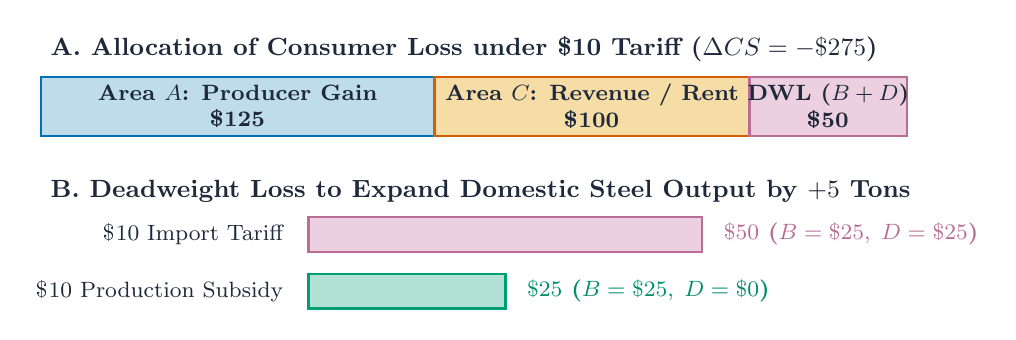
\begin{tikzpicture}[xscale=1.0, yscale=1.0]
    % Panel 1: Decomposition of $275 Consumer Loss under $10 Tariff (Horizontal stacked bar)
    \node[anchor=west, font=\small\bfseries, color=SlateBlue] at (0, 3.35) {A. Allocation of Consumer Loss under \$10 Tariff ($\Delta CS = -\$275$)};

    % Scale: 1 cm = $25 -> $125 = 5.0 cm, $100 = 4.0 cm, $50 = 2.0 cm (Total = 11.0 cm)
    \fill[CourseBlue!25, draw=CourseBlue, thick] (0, 2.25) rectangle (5.0, 3.0);
    \node[font=\footnotesize\bfseries, color=SlateBlue, align=center] at (2.5, 2.625) {Area $A$: Producer Gain\\ \$125};

    \fill[CourseAmber!35, draw=CourseOrange, thick] (5.0, 2.25) rectangle (9.0, 3.0);
    \node[font=\footnotesize\bfseries, color=SlateBlue, align=center] at (7.0, 2.625) {Area $C$: Revenue / Rent\\ \$100};

    \fill[CoursePurple!35, draw=CoursePurple!90!black, thick] (9.0, 2.25) rectangle (11.0, 3.0);
    \node[font=\footnotesize\bfseries, color=SlateBlue, align=center] at (10.0, 2.625) {DWL ($B+D$)\\ \$50};

    % Panel 2: Deadweight Loss Comparison for Expanding Domestic Output by +5 Tons
    \node[anchor=west, font=\small\bfseries, color=SlateBlue] at (0, 1.55) {B. Deadweight Loss to Expand Domestic Steel Output by $+5$ Tons};

    % Tariff DWL bar: $50 -> 5.0 cm (scale 1 cm = $10 for panel B)
    \node[anchor=east, font=\footnotesize, color=SlateBlue] at (3.2, 1.0) {\$10 Import Tariff};
    \fill[CoursePurple!35, draw=CoursePurple!90!black, thick] (3.4, 0.78) rectangle (8.4, 1.22);
    \node[anchor=west, font=\footnotesize\bfseries, color=CoursePurple!90!black] at (8.55, 1.0) {$\$50$ ($B = \$25,\; D = \$25$)};

    % Subsidy DWL bar: $25 -> 2.5 cm
    \node[anchor=east, font=\footnotesize, color=SlateBlue] at (3.2, 0.28) {\$10 Production Subsidy};
    \fill[CourseTeal!30, draw=CourseTeal, thick] (3.4, 0.06) rectangle (5.9, 0.50);
    \node[anchor=west, font=\footnotesize\bfseries, color=CourseTeal!90!black] at (6.05, 0.28) {$\$25$ ($B = \$25,\; D = \$0$)};
\end{tikzpicture}
\caption{Policy Evaluation of the $\$10$ Steel Tariff. Panel A decomposes the $\$275$ consumer loss into producer transfers ($\$125$), tariff revenue or quota rents ($\$100$), and deadweight loss ($\$50$). Panel B shows that a $\$10$ domestic production subsidy achieves the exact same $+5$-ton domestic output increase while eliminating consumption deadweight loss (Triangle $D$), halving total deadweight loss to $\$25$.}
\label{fig:tariff_vs_subsidy_policy}
\end{figure}

\subsection*{Mathematical Foundation (Algebra-First)}
To evaluate the economic efficiency of job-protection arguments, economists divide the consumer burden and deadweight loss of a trade barrier by the number of domestic jobs protected ($\Delta L_{\text{protected}}$):
\begin{equation}
\text{Consumer Cost per Job Protected} = \frac{|\Delta CS|}{\Delta L_{\text{protected}}}, \qquad \text{Deadweight Loss per Job Protected} = \frac{B + D}{\Delta L_{\text{protected}}}
\end{equation}

\begin{tcolorbox}[colback=LightSlate,colframe=CourseBlue,title=\textbf{Work It Out 14.3: Calculating Consumer Cost per Job Protected}]
Suppose our steel market in Work It Out 14.2 is scaled to \textbf{thousands of tons} ($P$ remains in dollars per ton), so the $\$10$ per-unit tariff expands domestic production by $\Delta Q_s = 5{,}000$ tons, reduces Consumer Surplus by $|\Delta CS| = \$275{,}000$, raises Producer Surplus by $\$125{,}000$, generates $\$100{,}000$ in tariff revenue, and creates $\$50{,}000$ in deadweight loss. Assume, as a hypothetical illustration, that producing those extra $5{,}000$ tons preserves $\Delta L_{\text{protected}} = 5$ domestic steelworker jobs.
\begin{enumerate}
    \item Calculate the \textbf{consumer cost per job protected}.
    \item Calculate the \textbf{producer surplus gain per job protected} and the \textbf{pure deadweight loss per job protected}.
    \item Interpret why consumers pay substantially more per job than domestic steel producers receive.
\end{enumerate}

\medskip
\noindent\textbf{Step-by-Step Solution:}
\begin{enumerate}
    \item \textbf{Consumer Cost per Job Protected:}
    \[
    \frac{|\Delta CS|}{\Delta L_{\text{protected}}} = \frac{\$275{,}000}{5\text{ jobs}} = \mathbf{\$55{,}000\text{ per job}}
    \]

    \item \textbf{Producer Surplus Gain and Deadweight Loss per Job Protected:}
    \[
    \text{Producer Surplus Gain per Job} = \frac{\$125{,}000}{5} = \mathbf{\$25{,}000\text{ per job}}
    \]
    \[
    \text{Deadweight Loss per Job} = \frac{\$50{,}000}{5} = \mathbf{\$10{,}000\text{ per job}}
    \]

    \item \textbf{Economic Interpretation:}
    Consumers bear $\$55{,}000$ in higher steel costs for every protected job, yet only $\$25{,}000$ reaches domestic steel producers as surplus (while $\$20{,}000$ goes to tariff revenue and $\$10{,}000$ vanishes into deadweight loss). Moreover, if higher steel prices eliminate jobs in downstream industries such as auto manufacturing, the net domestic employment gain is even smaller.
\end{enumerate}
\end{tcolorbox}

\begin{tcolorbox}[colback=SlateBlue!5!white,colframe=SlateBlue,title=\textbf{Optional Advanced Calculus Extension: The Targeting Principle (Subsidy vs. Tariff)}]
\small
\emph{Note for Economics Majors and Quantitative Students:}
Suppose policymakers seek to raise domestic steel production from $Q_{s1} = 10$ to $Q_{s2} = 15$ tons for national security. Instead of a $\$10$ tariff, consider a direct domestic production subsidy of $s = \$10$ per ton. Domestic firms receive $P_w + s = \$50$ and produce $15$ tons ($\Delta PS = +\$125$), while domestic consumers still pay $P_w = \$40$ and buy $30$ tons ($\Delta CS = \$0$). Government subsidy expenditure is $s \times Q_{s2} = \$10 \times 15 = \$150$, so net social surplus changes by:
\[
\Delta TS_{\text{subsidy}} = \Delta CS + \Delta PS - s Q_{s2} = 0 + \$125 - \$150 = -\$25 = -\text{Area } B.
\]
More generally, differentiating total surplus with respect to a tariff $t$ versus a production subsidy $s$ shows that marginal deadweight loss satisfies:
\[
\frac{d(DWL_{\text{tariff}})}{dt} = t\bigl[Q_s'(P_w + t) - Q_d'(P_w + t)\bigr] \;>\; s\,Q_s'(P_w + s) = \frac{d(DWL_{\text{subsidy}})}{ds} \quad (\text{at } t = s > 0, \text{ since } Q_d' < 0).
\]
Because the subsidy directly targets the production goal without raising the consumer price, it eliminates consumption distortion Triangle $D$ and strictly dominates the tariff in welfare terms.
\end{tcolorbox}

\begin{examplecase}{Bring It Home: Weighing Concentrated Producer Gains Against Dispersed Consumer Costs}
Returning to the debate between domestic steelworkers and automakers, our surplus framework reveals why trade disputes are so hard to resolve politically. A steel tariff delivers immediate, visible producer gains (Area $A$) to domestic mills and their workforce, while spreading a larger consumer loss ($A + B + C + D$) across millions of households and downstream manufacturers. Because society as a whole loses deadweight loss ($B + D$)---and loses even more ($B + C + D$) if an import quota hands quota rents to foreign exporters---economists generally recommend keeping trade open while supporting displaced workers directly through retraining and adjustment policies rather than restricting imports.
\end{examplecase}

\begin{takeaways}
\boxheader{SlateBlue}{Key Takeaways}
\begin{itemize}
    \item \textbf{Comparative Advantage Drives Trade Direction:} A small open economy imports when $P_w < P_A$ and exports when $P_w > P_A$. Both importing and exporting generate positive net gains in Total Social Surplus ($\Delta TS > 0$).
    \item \textbf{Trade Creates Winners and Losers:} Imports raise Consumer Surplus by more than Producer Surplus falls; exports raise Producer Surplus by more than Consumer Surplus falls.
    \item \textbf{Tariffs and Quotas Create Two DWL Triangles:} Both a per-unit tariff $t$ and an equivalent import quota raise the domestic price to $P_w + t$ and destroy surplus equal to production inefficiency ($B$) plus consumption inefficiency ($D$). Unlike tariff revenue, quota rents (Area $C$) accrue to license holders.
    \item \textbf{Targeting Beats Broad Protection:} Even when policymakers have a legitimate domestic production goal (such as national security), a direct production subsidy avoids consumer-side deadweight loss ($D$) and is strictly less costly to society than an import tariff.
\end{itemize}
\end{takeaways}

\end{document}
